%%
% BIThesis 实验报告模板 The BIThesis Template for Experiment Report
% This file has no copyright assigned and is placed in the Public Domain.
% Compile with: xelatex -> biber -> xelatex -> xelatex
%%

% 请勿删除下面两行注释,以免影响编译。
% !TeX program = xelatex
% !BIB program = biber

\documentclass[]{bitreport}

% 将你的相关信息替换如下示例
\BITSetup{
  cover = {
    % 在封面中载入有「北京理工大学销毁」的图片,如无必要请勿改动。
    imagePath = { assets/logo_bit.png },
    %% 使用以下参数来自定义封面日期
    date = {2026年01月11日}
  },
  info = {
    % 想要删除某项封面信息,直接删除该项即可。
    % 想要让某项封面信息留空(但是保留下划线),请传入空白符组成的字符串,如"{~}"。
    % 如需要换行,则用 "\\" 符号分割。
    title = {大数据泛构实验报告4\\多Pivot树状索引的实现与对比分析},
    school = {珠海校区},
    major = {计算机科学与技术},
    studentId = {3120256739},
    author = {丁纪翔},
    supervisor = {毛睿},
  }
}

%% 参考文献
\usepackage[style=gb7714-2015,backend=biber]{biblatex}
% Required by `figure`.
\usepackage{float,graphicx}
% Code listings
\usepackage{listings}
\usepackage{xcolor}
% Math symbols and environments
\usepackage{amsmath}
\usepackage{amssymb}
\usepackage{pifont}
% Algorithm packages
\usepackage{algorithm}
\usepackage{algorithmic}
% TikZ for drawing
\usepackage{tikz}
\usetikzlibrary{shapes,arrows,positioning,calc,trees,decorations.pathreplacing}
% PGFPlots for charts
\usepackage{pgfplots}
\pgfplotsset{compat=1.18}
% Multi-row and multi-column tables
\usepackage{multirow}
\usepackage{booktabs}
\usepackage{array}
% Subfigures
\usepackage{subcaption}

% 超链接支持(让目录可点击跳转)
\usepackage[
    colorlinks=true,      % 使用彩色链接
    linkcolor=blue,       % 内部链接颜色(目录、交叉引用等)
    citecolor=blue,       % 引用链接颜色
    urlcolor=blue,        % URL链接颜色
    bookmarksnumbered,    % PDF书签显示章节编号
    pdfstartview=FitH,    % PDF打开时适应页面宽度
]{hyperref}

% Java代码样式配置
\lstdefinestyle{javastyle}{
    language=Java,
    basicstyle=\ttfamily\small,
    keywordstyle=\color{blue}\bfseries,
    commentstyle=\color{gray}\itshape,
    stringstyle=\color{red},
    numbers=left,
    numberstyle=\tiny\color{gray},
    stepnumber=1,
    numbersep=8pt,
    backgroundcolor=\color{white},
    showspaces=false,
    showstringspaces=false,
    showtabs=false,
    frame=single,
    tabsize=4,
    captionpos=b,
    breaklines=true,
    breakatwhitespace=false,
    escapeinside={\%*}{*)},
    xleftmargin=2em,
    xrightmargin=2em,
    aboveskip=1em,
    belowskip=1em
}

\lstset{style=javastyle}

% 伪代码样式
\lstdefinestyle{pseudocode}{
    basicstyle=\ttfamily\small,
    keywordstyle=\color{blue}\bfseries,
    commentstyle=\color{gray}\itshape,
    numbers=left,
    numberstyle=\tiny\color{gray},
    stepnumber=1,
    numbersep=8pt,
    frame=single,
    tabsize=4,
    breaklines=true,
    xleftmargin=2em,
    xrightmargin=2em,
    aboveskip=1em,
    belowskip=1em,
    morekeywords={function,if,else,return,for,each,in,while,do,end,then,AND,OR,NOT,to}
}

% 算法环境配置
\renewcommand{\algorithmicrequire}{\textbf{Input:}}
\renewcommand{\algorithmicensure}{\textbf{Output:}}

\addbibresource{misc/refs.bib}

% 设置PDF文档属性
\hypersetup{
    pdftitle={大数据泛构实验报告4},
    pdfauthor={丁纪翔},
    pdfsubject={大数据实验报告},
    pdfkeywords={大数据, MVPT, CGHT, 完全线性划分, 度量空间索引}
}

% 定义一些常用命令
\newcommand{\ghTree}{GH-Tree}
\newcommand{\vpTree}{VP-Tree}
\newcommand{\mvpTree}{MVP-Tree}
\newcommand{\cghTree}{CGH-Tree}
\newcommand{\lpTree}{LP-Tree}
\newcommand{\cmark}{\ding{51}}
\newcommand{\xmark}{\ding{55}}

\begin{document}

% 制作封面
\MakeCover

% 生成目录
\tableofcontents
\clearpage

% 引入各章节内容
% Chapter 1: Introduction
\section{引言}

\subsection{研究背景与意义}

度量空间(Metric Space)是一种通用的数据抽象方式,可以涵盖向量、字符串、图像、生物序列等多种数据类型。在度量空间中,数据对象之间的相似性通过满足正定性、对称性和三角不等式的距离函数来度量。相似性查询是度量空间数据管理中最基本的操作之一,包括范围查询(Range Query)和k近邻查询(kNN Query)。

随着大数据时代的到来,如何高效地处理海量度量空间数据成为重要的研究课题。线性扫描方法虽然简单,但时间复杂度为$O(n)$,无法满足大规模数据集的查询需求。因此,设计高效的索引结构来加速相似性查询具有重要的理论意义和实际价值。

树状索引是度量空间索引的重要类别,通过层次化的数据划分实现高效的剪枝,可以显著减少查询时的距离计算次数。GH树(Generalized Hyperplane Tree)和VP树(Vantage Point Tree)是两种经典的树状索引结构,分别采用超平面划分和球形划分策略。

\subsection{任务回顾与目标}

\subsubsection{Assignment 1 \& 2 工作简述}

在Assignment 1中,我们建立了度量空间数据管理的基础设施,包括:
\begin{itemize}
    \item 核心抽象类:\texttt{MetricSpaceData}和\texttt{MetricFunction}
    \item 具体数据类型:向量数据(\texttt{VectorData})和蛋白质序列(\texttt{ProteinData})
    \item 距离函数实现:闵可夫斯基距离和Alignment距离
    \item 数据读取模块:支持从文件读取向量和蛋白质序列数据
\end{itemize}

在Assignment 2中,我们实现了基础的查询算法和Pivot Table索引:
\begin{itemize}
    \item 线性扫描查询:范围查询、kNN查询、多样化kNN查询
    \item Pivot Table索引:利用支撑点预计算距离实现查询剪枝
    \item Pivot选择策略:随机选择、FFT、增量选择等
\end{itemize}

\subsubsection{Assignment 3 核心目标}

本次Assignment 3的核心目标是实现两种树状度量空间索引——GH树和VP树,并进行全面的性能对比分析。具体任务包括:

\begin{enumerate}
    \item \textbf{代码实现}:实现GH树和VP树的数据结构、批建算法、范围查询和kNN查询
    \item \textbf{实验设计}:设计科学的性能对比实验方案,包括评价指标、数据集选择、参数设置等
    \item \textbf{正确性验证}:通过与线性扫描对比、手工验证等方式证明实现的正确性
    \item \textbf{性能对比}:在多种数据集上对比GH树和VP树的性能
    \item \textbf{分析讨论}:分析性能差异的原因,总结两种索引的优缺点,讨论改进方向
\end{enumerate}

\subsection{实验环境}

本实验的软硬件环境如表\ref{tab:environment}所示。

\begin{table}[htbp]
    \centering
    \caption{实验环境配置}
    \label{tab:environment}
    \begin{tabular}{ll}
        \toprule
        \textbf{项目} & \textbf{配置} \\
        \midrule
        操作系统 & Windows 11 \\
        CPU & Intel Core \\
        内存 & 16GB \\
        编程语言 & Java 11 \\
        构建工具 & Maven 3.8+ \\
        IDE & VS Code \\
        \bottomrule
    \end{tabular}
\end{table}

\subsection{报告结构}

本报告的组织结构如下:

\begin{itemize}
    \item \textbf{第2章 树状度量空间索引理论基础}:介绍GH树和VP树的基本概念、数据结构和算法原理
    \item \textbf{第3章 GHT和VPT实现}:详细描述系统架构扩展和核心算法的实现
    \item \textbf{第4章 功能正确性验证}:通过小规模数据演示和与线性扫描对比验证实现的正确性
    \item \textbf{第5章 性能对比实验设计与实施}:设计实验方案并在多种数据集上进行实验
    \item \textbf{第6章 性能对比分析}:分析实验结果,讨论性能差异的原因和改进方向
    \item \textbf{第7章 总结与展望}:总结本次工作,展望未来研究方向
\end{itemize}

本项目的完整代码已上传至GitHub仓库:

\url{https://github.com/sylvanding/BigDataGenhierarchy_Jixiang_20251116}


% Chapter 2: Theory
\section{理论基础}

\subsection{度量空间与支撑点空间}

\subsubsection{度量空间回顾}

度量空间是一个二元组$(M, d)$,其中$M$是数据对象的集合,$d: M \times M \to \mathbb{R}^+_0$是距离函数,满足:
\begin{itemize}
    \item \textbf{正定性}:$d(x, y) \geq 0$,当且仅当$x = y$时$d(x, y) = 0$
    \item \textbf{对称性}:$d(x, y) = d(y, x)$
    \item \textbf{三角不等式}:$d(x, z) \leq d(x, y) + d(y, z)$
\end{itemize}

\subsubsection{支撑点空间定义}

给定度量空间$(M, d)$和$k$个支撑点$P = \{p_1, p_2, ..., p_k\}$,\textbf{支撑点空间映射}定义为:
\begin{equation}
    F_d^P: M \to \mathbb{R}^k: x^P = F_d^P(x) = (d(x, p_1), d(x, p_2), ..., d(x, p_k))
\end{equation}

对于3个pivot,数据被映射到3维空间:$(d_1, d_2, d_3) = (d(x, p_1), d(x, p_2), d(x, p_3))$。

\subsubsection{支撑点空间的性质}

\textbf{性质1(距离下界)}:对于度量空间中的任意两点$x, y$:
\begin{equation}
    d(x, y) \geq \max_{i} |d(x, p_i) - d(y, p_i)| = d_{\infty}(x^P, y^P)
\end{equation}

即度量空间距离是支撑点空间切比雪夫距离的上界。

\textbf{性质2(范围查询映射)}:度量空间中以$q$为中心、半径$r$的范围查询,映射到支撑点空间后:
\begin{itemize}
    \item 包含于以$q^P$为中心、半径$r$的切比雪夫球中
    \item 即一个边长$2r$的超立方体$\{x^P: \max_i |x_i^P - q_i^P| \leq r\}$
\end{itemize}

\subsection{MVP树原理}

\subsubsection{基本思想}

MVP树(Multiple Vantage Point Tree)由Bozkaya和Ozsoyoglu于1999年提出,是VP树的自然扩展:
\begin{itemize}
    \item \textbf{VP树}:1个pivot,划分为2个部分,记为MVP(1,2)
    \item \textbf{MVP树}:$k$个pivot,每个pivot划分为$f$个部分,记为MVP(k,f)
\end{itemize}

对于MVP(3,2)树(本次实现):
\begin{itemize}
    \item 使用3个pivot:$p_1, p_2, p_3$
    \item 每个pivot将数据划分为2个部分(内球/外球)
    \item 总共产生$2^3 = 8$个子区域
\end{itemize}

\subsubsection{数据划分方式}

MVP树采用\textbf{嵌套球形划分}:
\begin{enumerate}
    \item 按第1个支撑点距离的中位数划分为2个子集
    \item 对每个子集,按第2个支撑点距离的中位数再划分
    \item 对每个子集,按第3个支撑点距离的中位数再划分
    \item 共得到8个子集
\end{enumerate}

子树索引使用二进制编码,如表\ref{tab:mvp-partition}所示。

\begin{table}[htbp]
    \centering
    \caption{MVP树子区域编码}
    \label{tab:mvp-partition}
    \begin{tabular}{ccccc}
        \toprule
        \textbf{Index} & \textbf{Binary} & \textbf{$p_1$ Region} & \textbf{$p_2$ Region} & \textbf{$p_3$ Region} \\
        \midrule
        0 & 000 & Inner & Inner & Inner \\
        1 & 001 & Outer & Inner & Inner \\
        2 & 010 & Inner & Outer & Inner \\
        3 & 011 & Outer & Outer & Inner \\
        4 & 100 & Inner & Inner & Outer \\
        5 & 101 & Outer & Inner & Outer \\
        6 & 110 & Inner & Outer & Outer \\
        7 & 111 & Outer & Outer & Outer \\
        \bottomrule
    \end{tabular}
\end{table}

\subsubsection{剪枝规则}

对于查询$(q, r)$和子树$i$,设:
\begin{itemize}
    \item $d_j = d(q, p_j)$:查询对象到第$j$个pivot的距离
    \item $[L_{i,j}, U_{i,j}]$:子树$i$中数据到第$j$个pivot的距离范围
\end{itemize}

\textbf{排除规则}(任一成立即可排除):
\begin{equation}
    \exists j: d_j + r < L_{i,j} \quad \text{或} \quad d_j - r > U_{i,j}
\end{equation}

\textbf{包含规则}(任一成立则全包含):
\begin{equation}
    \exists j: d_j + U_{i,j} \leq r
\end{equation}

图\ref{fig:mvp-partition}展示了MVP树的嵌套球形划分示意。

\begin{figure}[htbp]
    \centering
    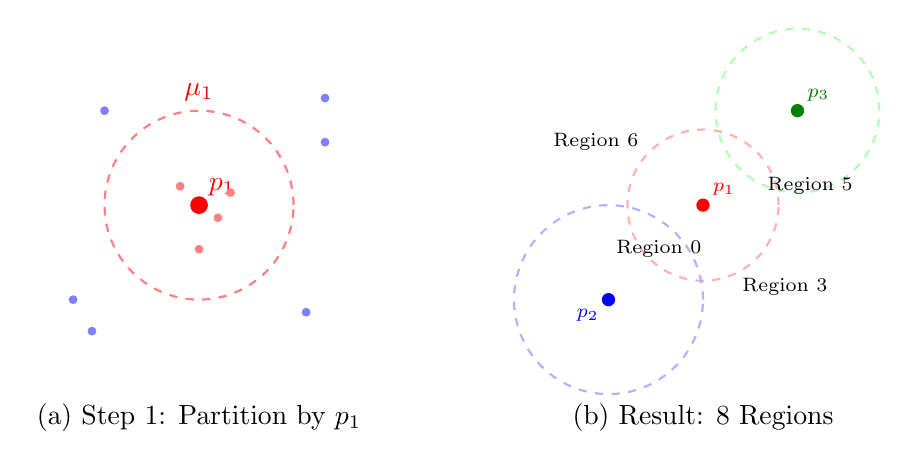
\begin{tikzpicture}[scale=0.8]
        % First pivot division
        \begin{scope}[xshift=0cm]
            \fill[red] (2.5,2.5) circle (4pt) node[above right] {$p_1$};
            \draw[thick,dashed,red!50] (2.5,2.5) circle (1.5);
            \node[red] at (2.5,4.3) {$\mu_1$};
            
            % Data points
            \foreach \x/\y in {2.2/2.8, 2.8/2.3, 2.5/1.8, 3/2.7} {
                \fill[red!50] (\x,\y) circle (2pt);
            }
            \foreach \x/\y in {0.5/1, 4.5/3.5, 1/4, 4.2/0.8, 0.8/0.5, 4.5/4.2} {
                \fill[blue!50] (\x,\y) circle (2pt);
            }
            
            \node[below] at (2.5,-0.5) {(a) Step 1: Partition by $p_1$};
        \end{scope}
        
        % After all three partitions
        \begin{scope}[xshift=8cm]
            \fill[red] (2.5,2.5) circle (3pt) node[above right] {\scriptsize $p_1$};
            \fill[blue] (1,1) circle (3pt) node[below left] {\scriptsize $p_2$};
            \fill[green!50!black] (4,4) circle (3pt) node[above right] {\scriptsize $p_3$};
            
            % Concentric circles (conceptual)
            \draw[thick,dashed,red!30] (2.5,2.5) circle (1.2);
            \draw[thick,dashed,blue!30] (1,1) circle (1.5);
            \draw[thick,dashed,green!30] (4,4) circle (1.3);
            
            % Data regions (simplified)
            \node at (1.8,1.8) {\scriptsize Region 0};
            \node at (3.8,1.2) {\scriptsize Region 3};
            \node at (0.8,3.5) {\scriptsize Region 6};
            \node at (4.2,2.8) {\scriptsize Region 5};
            
            \node[below] at (2.5,-0.5) {(b) Result: 8 Regions};
        \end{scope}
    \end{tikzpicture}
    \caption{MVP树嵌套球形划分示意}
    \label{fig:mvp-partition}
\end{figure}

\subsection{完全广义超平面树原理}

\subsubsection{基本思想}

完全广义超平面树(Complete GHT, CGHT)由毛睿教授于2014年提出,核心思想是:

\begin{quote}
    \textbf{充分利用pivot对之间的距离差信息进行划分}
\end{quote}

对于2个pivot $p_1, p_2$,原始GH树只利用了$d(x, p_1) - d(x, p_2)$的\textbf{符号}(正/负),而CGHT还利用其\textbf{大小}。

对于3个pivot,定义:
\begin{align}
    \delta_{12} &= d(x, p_1) - d(x, p_2) \\
    \delta_{13} &= d(x, p_1) - d(x, p_3) \\
    \delta_{23} &= d(x, p_2) - d(x, p_3) = \delta_{13} - \delta_{12}
\end{align}

只需要2个独立变量$(\delta_{12}, \delta_{13})$即可表示所有距离差信息。

\subsubsection{4路划分策略}

基于$\delta_{12}$和$\delta_{13}$的符号进行4路划分,如表\ref{tab:cgh-partition}所示。

\begin{table}[htbp]
    \centering
    \caption{CGH树4路划分}
    \label{tab:cgh-partition}
    \begin{tabular}{cccl}
        \toprule
        \textbf{Index} & \textbf{$\delta_{12}$} & \textbf{$\delta_{13}$} & \textbf{Geometric Meaning} \\
        \midrule
        0 & $< 0$ & $< 0$ & Farthest from $p_1$ \\
        1 & $\geq 0$ & $< 0$ & Farthest from $p_3$ \\
        2 & $< 0$ & $\geq 0$ & Farthest from $p_2$ \\
        3 & $\geq 0$ & $\geq 0$ & Closest to $p_1$ \\
        \bottomrule
    \end{tabular}
\end{table}

\subsubsection{剪枝规则}

基于GH树剪枝规则的扩展。对于查询$(q, r)$,设:
\begin{align}
    \delta_{12}^q &= d(q, p_1) - d(q, p_2) \\
    \delta_{13}^q &= d(q, p_1) - d(q, p_3)
\end{align}

对于子树$i$,其$\delta_{12}$范围为$[L_{12}^i, U_{12}^i]$,$\delta_{13}$范围为$[L_{13}^i, U_{13}^i]$。

\textbf{排除条件}(任一成立即可排除):
\begin{equation}
    \delta_{12}^q - 2r > U_{12}^i \quad \text{或} \quad \delta_{12}^q + 2r < L_{12}^i
\end{equation}
\begin{equation}
    \delta_{13}^q - 2r > U_{13}^i \quad \text{或} \quad \delta_{13}^q + 2r < L_{13}^i
\end{equation}

图\ref{fig:cgh-partition}展示了CGH树的超平面划分示意。

\begin{figure}[htbp]
    \centering
    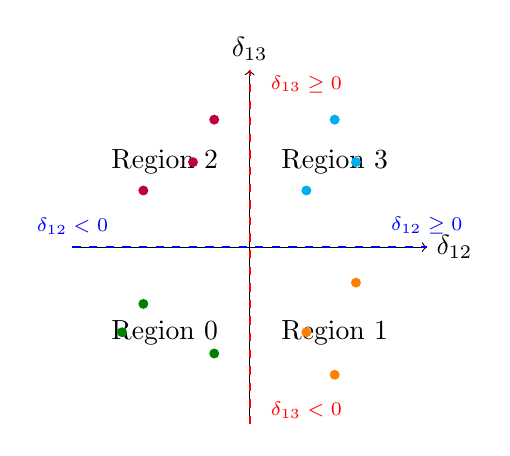
\begin{tikzpicture}[scale=0.9]
        % Coordinate system in delta space
        \draw[->] (-2.5,0) -- (2.5,0) node[right] {$\delta_{12}$};
        \draw[->] (0,-2.5) -- (0,2.5) node[above] {$\delta_{13}$};
        
        % Partition lines
        \draw[thick,dashed,blue] (-2.5,0) -- (2.5,0);
        \draw[thick,dashed,red] (0,-2.5) -- (0,2.5);
        
        % Regions
        \node at (-1.2,-1.2) {Region 0};
        \node at (1.2,-1.2) {Region 1};
        \node at (-1.2,1.2) {Region 2};
        \node at (1.2,1.2) {Region 3};
        
        % Annotations
        \node[blue] at (-2.5,0.3) {\scriptsize $\delta_{12} < 0$};
        \node[blue] at (2.5,0.3) {\scriptsize $\delta_{12} \geq 0$};
        \node[red] at (0.8,-2.3) {\scriptsize $\delta_{13} < 0$};
        \node[red] at (0.8,2.3) {\scriptsize $\delta_{13} \geq 0$};
        
        % Data points example
        \foreach \x/\y in {-1.5/-0.8, -0.5/-1.5, -1.8/-1.2} {
            \fill[green!50!black] (\x,\y) circle (2pt);
        }
        \foreach \x/\y in {0.8/-1.2, 1.5/-0.5, 1.2/-1.8} {
            \fill[orange] (\x,\y) circle (2pt);
        }
        \foreach \x/\y in {-0.8/1.2, -1.5/0.8, -0.5/1.8} {
            \fill[purple] (\x,\y) circle (2pt);
        }
        \foreach \x/\y in {0.8/0.8, 1.5/1.2, 1.2/1.8} {
            \fill[cyan] (\x,\y) circle (2pt);
        }
    \end{tikzpicture}
    \caption{CGH树在$(\delta_{12}, \delta_{13})$空间中的4路划分}
    \label{fig:cgh-partition}
\end{figure}

\subsection{完全线性划分原理}

\subsubsection{基本思想}

完全线性划分的核心思想是:

\begin{quote}
    既然数据已经映射到支撑点空间(多维实数空间),就可以使用传统的多维索引方法进行划分。
\end{quote}

\textbf{线性划分}:使用线性超平面$\sum_i a_i x_i = c$对支撑点空间进行划分。

最简单的线性划分是\textbf{正交划分}:
\begin{itemize}
    \item 按$d_1$的中位数划分
    \item 按$d_2$的中位数划分
    \item 按$d_3$的中位数划分
    \item 共产生$2^3 = 8$个子区域
\end{itemize}

\subsubsection{数据结构}

线性划分树内部节点存储:
\begin{itemize}
    \item 3个支撑点
    \item 3个维度的划分阈值(中位数)
    \item 8棵子树
    \item 每个子树在各维度的距离范围$[L_i^j, U_i^j]$
\end{itemize}

\subsubsection{剪枝规则}

查询对象在支撑点空间中的坐标为$q^P = (d_1^q, d_2^q, d_3^q)$。

查询区域是以$q^P$为中心的边长$2r$的立方体(切比雪夫球):
\begin{equation}
    \{(x_1, x_2, x_3): |x_i - d_i^q| \leq r, i=1,2,3\}
\end{equation}

\textbf{排除规则}:若存在任意维度$j$使得:
\begin{equation}
    d_j^q + r < L_i^j \quad \text{或} \quad d_j^q - r > U_i^j
\end{equation}
则子树$i$可以排除。

图\ref{fig:lp-partition}展示了线性划分树在支撑点空间中的划分。

\begin{figure}[htbp]
    \centering
    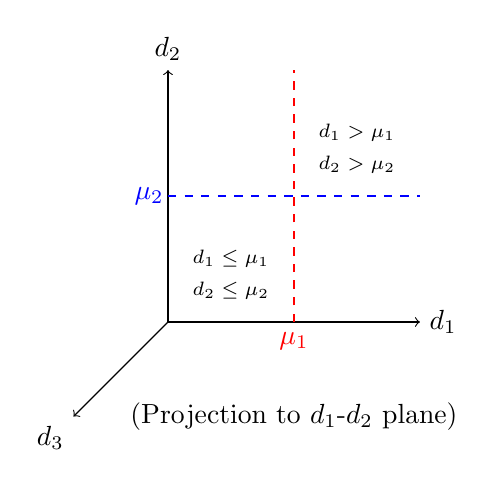
\begin{tikzpicture}[scale=0.8]
        % 3D coordinate system (isometric view)
        \draw[->] (0,0) -- (4,0) node[right] {$d_1$};
        \draw[->] (0,0) -- (0,4) node[above] {$d_2$};
        \draw[->] (0,0) -- (-1.5,-1.5) node[below left] {$d_3$};
        
        % Partition planes (simplified 2D projection)
        \draw[dashed,red] (2,0) -- (2,4);
        \draw[dashed,blue] (0,2) -- (4,2);
        
        % Threshold labels
        \node[red] at (2,-0.3) {$\mu_1$};
        \node[blue] at (-0.3,2) {$\mu_2$};
        
        % Regions
        \node at (1,1) {\scriptsize $d_1 \leq \mu_1$};
        \node at (1,0.5) {\scriptsize $d_2 \leq \mu_2$};
        \node at (3,3) {\scriptsize $d_1 > \mu_1$};
        \node at (3,2.5) {\scriptsize $d_2 > \mu_2$};
        
        % Note
        \node at (2,-1.5) {(Projection to $d_1$-$d_2$ plane)};
    \end{tikzpicture}
    \caption{线性划分树在支撑点空间中的正交划分($d_1$-$d_2$平面投影)}
    \label{fig:lp-partition}
\end{figure}

\subsection{三种索引的理论对比}

表\ref{tab:theory-compare}从多个维度对比了三种索引的特性。

\begin{table}[htbp]
    \centering
    \caption{三种多Pivot索引的理论对比}
    \label{tab:theory-compare}
    \begin{tabular}{lccc}
        \toprule
        \textbf{Feature} & \textbf{MVP Tree} & \textbf{CGH Tree} & \textbf{LP Tree} \\
        \midrule
        Partition Space & Metric Space & Metric Space & Pivot Space \\
        Partition Boundary & Spheres & Hyperplanes & Linear Hyperplanes \\
        Number of Children & $2^k = 8$ & $2^{k-1} = 4$ & $2^k = 8$ \\
        Distance Info Used & $d(x, p_i)$ & $d(x, p_i) - d(x, p_j)$ & $(d_1, d_2, d_3)$ \\
        Containment Rule & Yes & No & Yes (approx.) \\
        \bottomrule
    \end{tabular}
\end{table}

% Chapter 3: Implementation
\section{算法实现}

\subsection{系统架构}

\subsubsection{Assignment 4新增模块}

在Assignment 3的基础上,我们扩展系统架构以支持多Pivot树索引。图\ref{fig:architecture-a4}展示了扩展后的系统模块关系。

\begin{figure}[htbp]
    \centering
    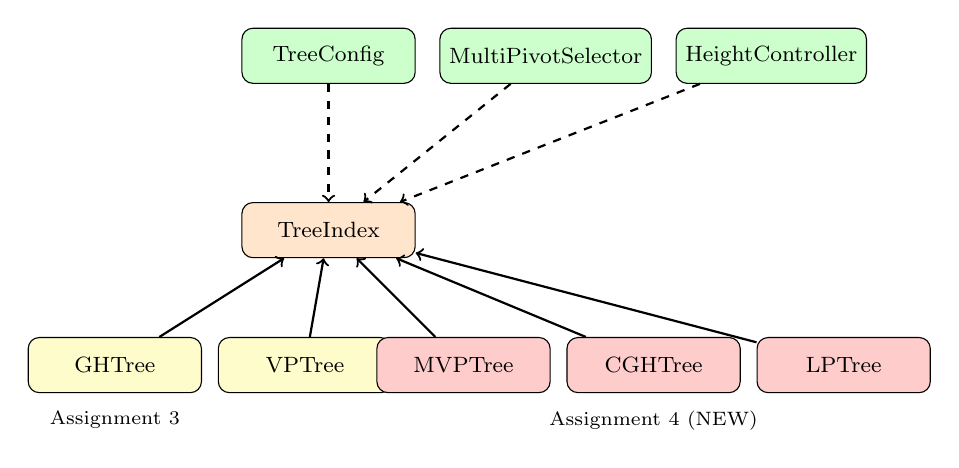
\begin{tikzpicture}[
        node distance=1cm,
        box/.style={rectangle, draw, rounded corners, minimum width=2.2cm, minimum height=0.7cm, text centered, font=\footnotesize},
        arrow/.style={->, thick}
    ]
        % Tree Index base
        \node[box, fill=orange!20] (treeindex) {TreeIndex};
        
        % Assignment 3 trees
        \node[box, fill=yellow!20, below left=1cm and 0.5cm of treeindex] (ghtree) {GHTree};
        \node[box, fill=yellow!20, right=0.2cm of ghtree] (vptree) {VPTree};
        
        % Assignment 4 trees
        \node[box, fill=red!20, below right=1cm and -0.5cm of treeindex] (mvptree) {MVPTree};
        \node[box, fill=red!20, right=0.2cm of mvptree] (cghtree) {CGHTree};
        \node[box, fill=red!20, right=0.2cm of cghtree] (lptree) {LPTree};
        
        % Common components
        \node[box, fill=green!20, above=1.5cm of treeindex] (config) {TreeConfig};
        \node[box, fill=green!20, right=0.3cm of config] (selector) {MultiPivotSelector};
        \node[box, fill=green!20, right=0.3cm of selector] (controller) {HeightController};
        
        % Arrows
        \draw[arrow] (ghtree) -- (treeindex);
        \draw[arrow] (vptree) -- (treeindex);
        \draw[arrow] (mvptree) -- (treeindex);
        \draw[arrow] (cghtree) -- (treeindex);
        \draw[arrow] (lptree) -- (treeindex);
        
        \draw[arrow,dashed] (config) -- (treeindex);
        \draw[arrow,dashed] (selector) -- (treeindex);
        \draw[arrow,dashed] (controller) -- (treeindex);
        
        % Labels
        \node[below=0.1cm of ghtree, font=\scriptsize] {Assignment 3};
        \node[below=0.1cm of cghtree, font=\scriptsize] {Assignment 4 (NEW)};
    \end{tikzpicture}
    \caption{Assignment 4系统架构扩展}
    \label{fig:architecture-a4}
\end{figure}

表\ref{tab:new-modules}展示了Assignment 4新增的主要模块。

\begin{table}[htbp]
    \centering
    \caption{Assignment 4新增模块}
    \label{tab:new-modules}
    \begin{tabular}{ll}
        \toprule
        \textbf{Module/Class} & \textbf{Description} \\
        \midrule
        \texttt{MultiPivotSelector} & Multi-pivot selection with FFT/RANDOM/MAX\_SPREAD \\
        \texttt{mvptree.MVPTree} & 3-pivot MVP tree implementation \\
        \texttt{mvptree.MVPInternalNode} & MVP tree internal node \\
        \texttt{cght.CGHTree} & 3-pivot CGH tree implementation \\
        \texttt{cght.CGHInternalNode} & CGH tree internal node \\
        \texttt{linearpartition.LinearPartitionTree} & 3-pivot linear partition tree \\
        \texttt{linearpartition.LPInternalNode} & Linear partition tree internal node \\
        \bottomrule
    \end{tabular}
\end{table}

\subsection{3-pivot MVPT实现}

\subsubsection{数据结构}

MVP树内部节点的核心数据结构如下:

\begin{lstlisting}[caption=MVPInternalNode数据结构]
public class MVPInternalNode extends InternalNode {
    private MetricSpaceData[] pivots;      // 3 pivots
    private TreeNode[] children;            // 8 children
    private double[] splitRadius;           // 3 split radii (medians)
    private double[][] lowerBound;          // [8][3] lower bounds
    private double[][] upperBound;          // [8][3] upper bounds
    
    public int getChildIndex(double d1, double d2, double d3) {
        int idx = 0;
        if (d1 > splitRadius[0]) idx |= 1;
        if (d2 > splitRadius[1]) idx |= 2;
        if (d3 > splitRadius[2]) idx |= 4;
        return idx;
    }
}
\end{lstlisting}

\subsubsection{批建算法}

MVP树批建算法的核心逻辑如算法\ref{alg:mvp-build}所示。

\begin{algorithm}[htbp]
    \caption{MVP树批建算法}
    \label{alg:mvp-build}
    \begin{algorithmic}[1]
        \REQUIRE 数据集$S$,当前深度$depth$
        \ENSURE MVP树节点
        \IF{$|S| \leq maxLeafSize$ \AND $depth \geq minTreeHeight$}
            \RETURN LeafNode($S$, $depth$)
        \ENDIF
        \STATE $(p_1, p_2, p_3) \leftarrow$ SelectThreePivots($S$)
        \STATE 计算所有数据到各pivot的距离
        \STATE $\mu_1, \mu_2, \mu_3 \leftarrow$ 各pivot维度的中位数
        \STATE 初始化8个子集 $partitions[0..7]$
        \FOR{each $x$ in $S - \{p_1, p_2, p_3\}$}
            \STATE $idx \leftarrow$ GetChildIndex($d(x,p_1), d(x,p_2), d(x,p_3)$)
            \STATE $partitions[idx]$.add($x$)
        \ENDFOR
        \STATE 计算每个子集的距离范围 $[L_{i,j}, U_{i,j}]$
        \FOR{$i = 0$ to $7$}
            \STATE $children[i] \leftarrow$ BuildMVPTree($partitions[i]$, $depth+1$)
        \ENDFOR
        \RETURN MVPInternalNode($pivots$, $children$, $bounds$)
    \end{algorithmic}
\end{algorithm}

\subsubsection{范围查询算法}

MVP树范围查询利用距离范围进行剪枝:

\begin{lstlisting}[caption=MVP树范围查询核心实现]
private void rangeQueryRecursive(TreeNode node, 
        MetricSpaceData q, double r, List<MetricSpaceData> result) {
    if (node.isLeaf()) {
        // Linear scan leaf data
        for (MetricSpaceData obj : ((LeafNode)node).getData()) {
            if (metric.getDistance(q, obj) <= r) {
                result.add(obj);
            }
        }
        return;
    }
    
    MVPInternalNode internal = (MVPInternalNode) node;
    double[] dq = new double[3];
    for (int j = 0; j < 3; j++) {
        dq[j] = metric.getDistance(q, internal.getPivot(j));
        if (dq[j] <= r) result.add(internal.getPivot(j));
    }
    
    // Check each child
    for (int i = 0; i < 8; i++) {
        if (internal.getChild(i) == null) continue;
        
        boolean canPrune = false;
        boolean fullyContained = false;
        
        for (int j = 0; j < 3; j++) {
            double L = internal.getLowerBound(i, j);
            double U = internal.getUpperBound(i, j);
            
            // Exclusion rule
            if (dq[j] + r < L || dq[j] - r > U) {
                canPrune = true;
                break;
            }
            // Containment rule
            if (dq[j] + U <= r) {
                fullyContained = true;
                break;
            }
        }
        
        if (fullyContained) {
            collectAllData(internal.getChild(i), result);
        } else if (!canPrune) {
            rangeQueryRecursive(internal.getChild(i), q, r, result);
        }
    }
}
\end{lstlisting}

\subsection{3-pivot CGHT实现}

\subsubsection{数据结构}

CGH树内部节点基于距离差进行划分:

\begin{lstlisting}[caption=CGHInternalNode数据结构]
public class CGHInternalNode extends InternalNode {
    private MetricSpaceData[] pivots;       // 3 pivots
    private TreeNode[] children;             // 4 children
    private double[][] delta12Range;         // [4][2]: min, max of delta12
    private double[][] delta13Range;         // [4][2]: min, max of delta13
    
    public int getChildIndex(double d1, double d2, double d3) {
        double delta12 = d1 - d2;
        double delta13 = d1 - d3;
        int idx = 0;
        if (delta12 >= 0) idx |= 1;
        if (delta13 >= 0) idx |= 2;
        return idx;
    }
}
\end{lstlisting}

\subsubsection{批建算法}

CGH树批建算法如算法\ref{alg:cgh-build}所示。

\begin{algorithm}[htbp]
    \caption{CGH树批建算法}
    \label{alg:cgh-build}
    \begin{algorithmic}[1]
        \REQUIRE 数据集$S$,当前深度$depth$
        \ENSURE CGH树节点
        \IF{$|S| \leq maxLeafSize$ \AND $depth \geq minTreeHeight$}
            \RETURN LeafNode($S$, $depth$)
        \ENDIF
        \STATE $(p_1, p_2, p_3) \leftarrow$ SelectThreePivots($S$)
        \STATE 初始化4个子集 $partitions[0..3]$
        \FOR{each $x$ in $S - \{p_1, p_2, p_3\}$}
            \STATE $d_1, d_2, d_3 \leftarrow d(x, p_1), d(x, p_2), d(x, p_3)$
            \STATE $\delta_{12} \leftarrow d_1 - d_2$, $\delta_{13} \leftarrow d_1 - d_3$
            \STATE $idx \leftarrow$ ($\delta_{12} \geq 0$ ? 1 : 0) + ($\delta_{13} \geq 0$ ? 2 : 0)
            \STATE $partitions[idx]$.add($x$)
        \ENDFOR
        \STATE 计算每个子集的$\delta_{12}$和$\delta_{13}$范围
        \FOR{$i = 0$ to $3$}
            \STATE $children[i] \leftarrow$ BuildCGHTree($partitions[i]$, $depth+1$)
        \ENDFOR
        \RETURN CGHInternalNode($pivots$, $children$, $deltaRanges$)
    \end{algorithmic}
\end{algorithm}

\subsubsection{范围查询算法}

CGH树范围查询基于GH树剪枝规则的扩展:

\begin{lstlisting}[caption=CGH树范围查询核心实现]
private void rangeQueryRecursive(TreeNode node,
        MetricSpaceData q, double r, List<MetricSpaceData> result) {
    if (node.isLeaf()) {
        for (MetricSpaceData obj : ((LeafNode)node).getData()) {
            if (metric.getDistance(q, obj) <= r) {
                result.add(obj);
            }
        }
        return;
    }
    
    CGHInternalNode internal = (CGHInternalNode) node;
    double d1 = metric.getDistance(q, internal.getPivot(0));
    double d2 = metric.getDistance(q, internal.getPivot(1));
    double d3 = metric.getDistance(q, internal.getPivot(2));
    
    // Check pivots
    if (d1 <= r) result.add(internal.getPivot(0));
    if (d2 <= r) result.add(internal.getPivot(1));
    if (d3 <= r) result.add(internal.getPivot(2));
    
    double deltaQ12 = d1 - d2;
    double deltaQ13 = d1 - d3;
    
    // Check each child
    for (int i = 0; i < 4; i++) {
        if (internal.getChild(i) == null) continue;
        
        double[] range12 = internal.getDelta12Range(i);
        double[] range13 = internal.getDelta13Range(i);
        
        // Extended GH-tree pruning rule
        boolean canPrune = false;
        
        // Check delta12 range
        if (deltaQ12 - 2*r > range12[1] || deltaQ12 + 2*r < range12[0]) {
            canPrune = true;
        }
        // Check delta13 range
        if (deltaQ13 - 2*r > range13[1] || deltaQ13 + 2*r < range13[0]) {
            canPrune = true;
        }
        
        if (!canPrune) {
            rangeQueryRecursive(internal.getChild(i), q, r, result);
        }
    }
}
\end{lstlisting}

\subsection{完全线性划分树实现}

\subsubsection{数据结构}

线性划分树在支撑点空间中使用正交划分:

\begin{lstlisting}[caption=LinearPartitionInternalNode数据结构]
public class LinearPartitionInternalNode extends InternalNode {
    private MetricSpaceData[] pivots;       // 3 pivots
    private TreeNode[] children;             // 8 children
    private double[] splitThreshold;         // 3 thresholds (medians)
    private double[][] lowerBound;           // [8][3] coordinate lower bounds
    private double[][] upperBound;           // [8][3] coordinate upper bounds
    
    public int getChildIndex(double d1, double d2, double d3) {
        int idx = 0;
        if (d1 > splitThreshold[0]) idx |= 1;
        if (d2 > splitThreshold[1]) idx |= 2;
        if (d3 > splitThreshold[2]) idx |= 4;
        return idx;
    }
}
\end{lstlisting}

\subsubsection{批建算法}

线性划分树批建算法与MVP树类似,但在支撑点空间中进行划分。

\subsubsection{范围查询算法}

线性划分树范围查询在支撑点空间中判断立方体相交:

\begin{lstlisting}[caption=线性划分树范围查询核心实现]
private void rangeQueryRecursive(TreeNode node,
        MetricSpaceData q, double r, List<MetricSpaceData> result) {
    if (node.isLeaf()) {
        for (MetricSpaceData obj : ((LeafNode)node).getData()) {
            if (metric.getDistance(q, obj) <= r) {
                result.add(obj);
            }
        }
        return;
    }
    
    LPInternalNode internal = (LPInternalNode) node;
    double[] dq = new double[3];
    for (int j = 0; j < 3; j++) {
        dq[j] = metric.getDistance(q, internal.getPivot(j));
        if (dq[j] <= r) result.add(internal.getPivot(j));
    }
    
    // Query region is a cube: [dq[j]-r, dq[j]+r] for each j
    for (int i = 0; i < 8; i++) {
        if (internal.getChild(i) == null) continue;
        
        boolean canPrune = false;
        for (int j = 0; j < 3; j++) {
            double L = internal.getLowerBound(i, j);
            double U = internal.getUpperBound(i, j);
            
            // Check if query cube intersects with child region
            if (dq[j] + r < L || dq[j] - r > U) {
                canPrune = true;
                break;
            }
        }
        
        if (!canPrune) {
            rangeQueryRecursive(internal.getChild(i), q, r, result);
        }
    }
}
\end{lstlisting}

\subsection{统一的支撑点选择策略}

为了公平对比,三种索引使用统一的\texttt{MultiPivotSelector}选择支撑点:

\begin{lstlisting}[caption=MultiPivotSelector实现]
public class MultiPivotSelector {
    public enum SelectionStrategy { RANDOM, FFT, MAX_SPREAD }
    
    public MetricSpaceData[] selectPivots(
            List<? extends MetricSpaceData> data, 
            int numPivots,
            MetricFunction metric) {
        switch (strategy) {
            case RANDOM:
                return selectRandomPivots(data, numPivots);
            case FFT:
                return selectFFTPivots(data, numPivots, metric);
            case MAX_SPREAD:
                return selectMaxSpreadPivots(data, numPivots, metric);
            default:
                return selectFFTPivots(data, numPivots, metric);
        }
    }
    
    private MetricSpaceData[] selectFFTPivots(
            List<? extends MetricSpaceData> data, 
            int numPivots,
            MetricFunction metric) {
        MetricSpaceData[] pivots = new MetricSpaceData[numPivots];
        
        // First pivot: random
        pivots[0] = data.get(random.nextInt(data.size()));
        
        // Subsequent pivots: farthest from selected
        for (int i = 1; i < numPivots; i++) {
            double maxMinDist = -1;
            MetricSpaceData farthest = null;
            
            for (MetricSpaceData obj : data) {
                double minDist = Double.MAX_VALUE;
                for (int j = 0; j < i; j++) {
                    double d = metric.getDistance(obj, pivots[j]);
                    minDist = Math.min(minDist, d);
                }
                if (minDist > maxMinDist) {
                    maxMinDist = minDist;
                    farthest = obj;
                }
            }
            pivots[i] = farthest;
        }
        return pivots;
    }
}
\end{lstlisting}

\subsection{树配置与使用示例}

三种索引使用统一的配置方式:

\begin{lstlisting}[caption=多Pivot树索引使用示例]
// Configuration
TreeConfig config = new TreeConfig.Builder()
    .maxLeafSize(50)
    .minTreeHeight(2)
    .pivotStrategy(TreeConfig.PivotSelectionStrategy.FFT)
    .randomSeed(42)
    .verbose(false)
    .build();

// Create multi-pivot selector
MultiPivotSelector selector = new MultiPivotSelector(
    MultiPivotSelector.SelectionStrategy.FFT, 42);

// Build MVP Tree
MVPTree mvpTree = new MVPTree(config, selector);
mvpTree.buildIndex(dataset, new MinkowskiDistance(2));

// Build CGH Tree
CGHTree cghTree = new CGHTree(config, selector);
cghTree.buildIndex(dataset, new MinkowskiDistance(2));

// Build Linear Partition Tree
LinearPartitionTree lpTree = new LinearPartitionTree(config, selector);
lpTree.buildIndex(dataset, new MinkowskiDistance(2));

// Range Query
List<MetricSpaceData> results = mvpTree.rangeQuery(queryObj, radius);

// kNN Query
List<MetricSpaceData> knnResults = cghTree.knnQuery(queryObj, k);
\end{lstlisting}

% Chapter 4: Correctness Verification
\section{正确性验证}

\subsection{测试数据集}

为了验证三种多Pivot树索引的正确性,我们使用以下测试数据集:

\subsubsection{小规模2D向量数据集}

用于手工验证的小规模数据集,包含15个2维点:

\begin{table}[htbp]
    \centering
    \caption{小规模测试数据集}
    \label{tab:test-dataset}
    \begin{tabular}{ccc|ccc}
        \toprule
        \textbf{ID} & \textbf{x} & \textbf{y} & \textbf{ID} & \textbf{x} & \textbf{y} \\
        \midrule
        0 & 1.0 & 1.0 & 8 & 9.0 & 4.0 \\
        1 & 2.0 & 2.0 & 9 & 10.0 & 7.0 \\
        2 & 3.0 & 1.0 & 10 & 3.0 & 5.0 \\
        3 & 4.0 & 4.0 & 11 & 6.0 & 1.0 \\
        4 & 5.0 & 2.0 & 12 & 2.0 & 7.0 \\
        5 & 6.0 & 5.0 & 13 & 8.0 & 2.0 \\
        6 & 7.0 & 3.0 & 14 & 4.0 & 8.0 \\
        7 & 8.0 & 6.0 & & & \\
        \bottomrule
    \end{tabular}
\end{table}

\subsubsection{较大规模测试数据集}

用于综合测试的数据集:
\begin{itemize}
    \item 低维向量数据(2维):200个聚类分布点
    \item 高维向量数据(10维):500个均匀分布点
    \item 蛋白质序列数据:960条酵母蛋白质序列(长度6)
\end{itemize}

\subsection{各索引正确性验证}

\subsubsection{MVP树构建与查询验证}

使用小规模数据集验证MVP树的构建和查询正确性。

\textbf{构建结果}:
\begin{verbatim}
=== MVP Tree Build Result ===
Tree Height: 2
Total Nodes: 7
  - Internal Nodes: 3
  - Leaf Nodes: 4
Build Distance Computations: 84

Tree Structure:
└── MVP Internal [pivots=ID5,ID0,ID9, sizes=[2,0,5,0,1,4,0,0]]
    ├── Leaf [size=2]
    ├── MVP Internal [pivots=ID13,ID14,ID7, sizes=[2,0,0,0,0,0,0,0]]
    │   └── Leaf [size=2]
    ├── Leaf [size=1]
    └── MVP Internal [pivots=ID11,ID12,ID1, sizes=[1,0,0,0,0,0,0,0]]
        └── Leaf [size=1]
\end{verbatim}

\textbf{范围查询验证}(查询点(5.0, 5.0),半径3.0):

\begin{table}[htbp]
    \centering
    \caption{MVP树范围查询结果}
    \label{tab:mvp-range-result}
    \begin{tabular}{cccc}
        \toprule
        \textbf{ID} & \textbf{Coordinate} & \textbf{Distance} & \textbf{Result} \\
        \midrule
        5 & (6.0, 5.0) & 1.0000 & \cmark \\
        3 & (4.0, 4.0) & 1.4142 & \cmark \\
        10 & (3.0, 5.0) & 2.0000 & \cmark \\
        6 & (7.0, 3.0) & 2.8284 & \cmark \\
        4 & (5.0, 2.0) & 3.0000 & \cmark \\
        \bottomrule
    \end{tabular}
\end{table}

\subsubsection{CGH树构建与查询验证}

\textbf{构建结果}:
\begin{verbatim}
=== CGH Tree Build Result ===
Tree Height: 2
Total Nodes: 7
  - Internal Nodes: 2
  - Leaf Nodes: 5
Build Distance Computations: 91

Tree Structure:
└── CGH Internal [pivots=ID5,ID0,ID9, sizes=[8,2,2,0]]
    ├── CGH Internal [pivots=ID3,ID13,ID14, sizes=[2,2,1,0]]
    │   ├── Leaf [size=2]
    │   ├── Leaf [size=2]
    │   └── Leaf [size=1]
    ├── Leaf [size=2]
    └── Leaf [size=2]
\end{verbatim}

\textbf{范围查询验证}:结果与MVP树一致,查询距离计算次数为13次。

\subsubsection{线性划分树构建与查询验证}

\textbf{构建结果}:
\begin{verbatim}
=== Linear Partition Tree Build Result ===
Tree Height: 2
Total Nodes: 7
  - Internal Nodes: 3
  - Leaf Nodes: 4
Build Distance Computations: 84

Tree Structure:
└── LP Internal [pivots=ID5,ID0,ID9, sizes=[2,0,5,0,1,4,0,0]]
    ├── Leaf [size=2]
    ├── LP Internal [pivots=ID13,ID14,ID7, sizes=[2,0,0,0,0,0,0,0]]
    │   └── Leaf [size=2]
    ├── Leaf [size=1]
    └── LP Internal [pivots=ID11,ID12,ID1, sizes=[1,0,0,0,0,0,0,0]]
        └── Leaf [size=1]
\end{verbatim}

\textbf{范围查询验证}:结果与前两种索引一致,查询距离计算次数为15次。

\subsection{结果一致性验证}

\subsubsection{与线性扫描对比}

使用线性扫描作为基准,验证三种索引的查询结果一致性:

\begin{table}[htbp]
    \centering
    \caption{范围查询结果一致性验证}
    \label{tab:consistency-range}
    \begin{tabular}{lccc}
        \toprule
        \textbf{Method} & \textbf{Result Count} & \textbf{Distance Computations} & \textbf{Consistent} \\
        \midrule
        Linear Scan & 5 & 15 & - \\
        MVP Tree & 5 & 15 & \cmark \\
        CGH Tree & 5 & 13 & \cmark \\
        LP Tree & 5 & 15 & \cmark \\
        \bottomrule
    \end{tabular}
\end{table}

\subsubsection{kNN查询一致性验证}

对kNN查询(k=3)进行验证:

\begin{table}[htbp]
    \centering
    \caption{kNN查询结果一致性验证}
    \label{tab:consistency-knn}
    \begin{tabular}{lcccc}
        \toprule
        \textbf{Method} & \textbf{1st} & \textbf{2nd} & \textbf{3rd} & \textbf{Consistent} \\
        \midrule
        Linear Scan & ID5 (1.00) & ID3 (1.41) & ID10 (2.00) & - \\
        MVP Tree & ID5 (1.00) & ID3 (1.41) & ID10 (2.00) & \cmark \\
        CGH Tree & ID5 (1.00) & ID3 (1.41) & ID10 (2.00) & \cmark \\
        LP Tree & ID5 (1.00) & ID3 (1.41) & ID10 (2.00) & \cmark \\
        \bottomrule
    \end{tabular}
\end{table}

\subsubsection{大规模数据集验证}

在200个数据点的测试集上进行10轮随机查询验证:

\begin{table}[htbp]
    \centering
    \caption{大规模数据集验证结果}
    \label{tab:large-scale-verify}
    \begin{tabular}{lccc}
        \toprule
        \textbf{Index} & \textbf{Height} & \textbf{Nodes} & \textbf{Correctness} \\
        \midrule
        MVP Tree & 2 & 56 & 10/10 (100\%) \\
        CGH Tree & 5 & 55 & 10/10 (100\%) \\
        LP Tree & 2 & 56 & 10/10 (100\%) \\
        \bottomrule
    \end{tabular}
\end{table}

\subsection{单元测试结果}

运行\texttt{mvn test -Dtest=MultiPivotTreeTest},所有12个测试用例全部通过:

\begin{table}[htbp]
    \centering
    \caption{单元测试结果汇总}
    \label{tab:unit-test}
    \begin{tabular}{clc}
        \toprule
        \textbf{No.} & \textbf{Test Case} & \textbf{Status} \\
        \midrule
        1 & MVP Tree Build & \cmark \\
        2 & MVP Tree Range Query & \cmark \\
        3 & MVP Tree kNN Query & \cmark \\
        4 & CGH Tree Build & \cmark \\
        5 & CGH Tree Range Query & \cmark \\
        6 & CGH Tree kNN Query & \cmark \\
        7 & LP Tree Build & \cmark \\
        8 & LP Tree Range Query & \cmark \\
        9 & LP Tree kNN Query & \cmark \\
        10 & Three Index Consistency & \cmark \\
        11 & Large Dataset Test & \cmark \\
        12 & Empty Dataset Handling & \cmark \\
        \bottomrule
    \end{tabular}
\end{table}

测试运行时间:0.115秒,所有测试通过(Tests run: 12, Failures: 0, Errors: 0)。

\subsection{验证结论}

通过以上验证,我们确认:
\begin{enumerate}
    \item 三种多Pivot树索引均能正确构建,树结构符合预期
    \item 范围查询结果与线性扫描完全一致
    \item kNN查询结果与线性扫描完全一致
    \item 三种索引之间的结果相互一致
    \item 边界情况(空数据集)处理正确
\end{enumerate}

% Chapter 5: Theoretical Analysis
\section{理论对比分析}

\subsection{数据划分方式对比}

\subsubsection{划分空间与边界形状}

三种索引在数据划分方式上有本质区别,如表\ref{tab:partition-compare-detail}所示。

\begin{table}[htbp]
    \centering
    \caption{数据划分方式详细对比}
    \label{tab:partition-compare-detail}
    \begin{tabular}{lccc}
        \toprule
        \textbf{Aspect} & \textbf{MVP Tree} & \textbf{CGH Tree} & \textbf{LP Tree} \\
        \midrule
        Partition Space & Metric Space & Metric Space & Pivot Space \\
        Partition Method & Nested Spheres & Hyperplanes & Linear Hyperplanes \\
        Boundary Shape & Concentric Spheres & Distance Difference & Orthogonal Planes \\
        Number of Children & $2^k = 8$ & $2^{k-1} = 4$ & $2^k = 8$ \\
        Balance Guarantee & Median-based & Sign-based & Median-based \\
        \bottomrule
    \end{tabular}
\end{table}

\textbf{MVP树}:采用嵌套球形划分,每个pivot独立将数据分为内球和外球两部分。边界是以pivot为圆心的同心球面。

\textbf{CGH树}:采用超平面组合划分,基于距离差的符号进行划分。边界是由$\delta_{12}=0$和$\delta_{13}=0$定义的两个超平面。

\textbf{线性划分树}:在支撑点空间中采用正交划分,边界是与坐标轴垂直的超平面。

\subsubsection{划分平衡性分析}

\textbf{MVP树和LP树}:使用中位数进行划分,理论上保证每层划分的平衡性。但由于嵌套划分,后续层可能出现不平衡。

\textbf{CGH树}:基于距离差符号划分,平衡性依赖于数据分布。在某些分布下可能严重不平衡。

图\ref{fig:balance-analysis}展示了不同划分策略的平衡性特点。

\begin{figure}[htbp]
    \centering
    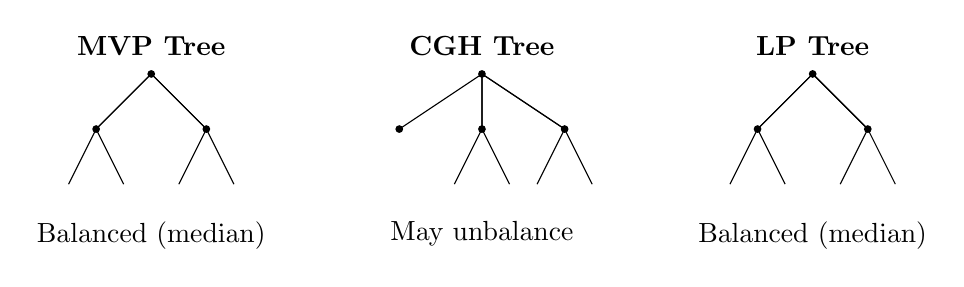
\begin{tikzpicture}[scale=0.7]
        % MVP Tree balance
        \begin{scope}[xshift=0cm]
            \node at (2,3.5) {\textbf{MVP Tree}};
            \draw (2,3) -- (1,2) -- (0.5,1);
            \draw (2,3) -- (1,2) -- (1.5,1);
            \draw (2,3) -- (3,2) -- (2.5,1);
            \draw (2,3) -- (3,2) -- (3.5,1);
            \fill (2,3) circle (2pt);
            \fill (1,2) circle (2pt);
            \fill (3,2) circle (2pt);
            \node[below] at (2,0.5) {Balanced (median)};
        \end{scope}
        
        % CGH Tree (potentially unbalanced)
        \begin{scope}[xshift=6cm]
            \node at (2,3.5) {\textbf{CGH Tree}};
            \draw (2,3) -- (0.5,2);
            \draw (2,3) -- (2,2) -- (1.5,1);
            \draw (2,3) -- (2,2) -- (2.5,1);
            \draw (2,3) -- (3.5,2) -- (3,1);
            \draw (2,3) -- (3.5,2) -- (4,1);
            \fill (2,3) circle (2pt);
            \fill (0.5,2) circle (2pt);
            \fill (2,2) circle (2pt);
            \fill (3.5,2) circle (2pt);
            \node[below] at (2,0.5) {May unbalance};
        \end{scope}
        
        % LP Tree balance
        \begin{scope}[xshift=12cm]
            \node at (2,3.5) {\textbf{LP Tree}};
            \draw (2,3) -- (1,2) -- (0.5,1);
            \draw (2,3) -- (1,2) -- (1.5,1);
            \draw (2,3) -- (3,2) -- (2.5,1);
            \draw (2,3) -- (3,2) -- (3.5,1);
            \fill (2,3) circle (2pt);
            \fill (1,2) circle (2pt);
            \fill (3,2) circle (2pt);
            \node[below] at (2,0.5) {Balanced (median)};
        \end{scope}
    \end{tikzpicture}
    \caption{三种索引的划分平衡性示意}
    \label{fig:balance-analysis}
\end{figure}

\subsection{支撑点使用效率对比}

\subsubsection{距离信息利用方式}

三种索引利用pivot距离信息的方式不同:

\begin{itemize}
    \item \textbf{MVP树}:独立使用每个pivot的距离值$d(x, p_i)$
    \item \textbf{CGH树}:使用pivot对的距离差$\delta_{ij} = d(x, p_i) - d(x, p_j)$
    \item \textbf{LP树}:联合使用距离向量$(d_1, d_2, d_3)$
\end{itemize}

\subsubsection{信息利用效率分析}

\textbf{MVP树}:每个pivot独立贡献剪枝信息,信息利用相对独立。剪枝条件是对各维度分别检查。

\textbf{CGH树}:利用pivot对之间的距离差,这包含了更多的相对位置信息。但只有$k-1$个独立的距离差变量。

\textbf{LP树}:在支撑点空间中统一利用所有距离信息,但映射过程可能导致信息损失(距离扭曲)。

\subsection{剪枝能力分析}

\subsubsection{剪枝条件对比}

表\ref{tab:pruning-compare}对比了三种索引的剪枝条件。

\begin{table}[htbp]
    \centering
    \caption{剪枝条件对比}
    \label{tab:pruning-compare}
    \begin{tabular}{ll}
        \toprule
        \textbf{Index} & \textbf{Pruning Condition} \\
        \midrule
        MVP Tree & $\exists j: d_j + r < L_{i,j}$ or $d_j - r > U_{i,j}$ \\
        CGH Tree & $\delta_{jk}^q - 2r > U_{jk}^i$ or $\delta_{jk}^q + 2r < L_{jk}^i$ \\
        LP Tree & $\exists j: d_j^q + r < L_i^j$ or $d_j^q - r > U_i^j$ \\
        \bottomrule
    \end{tabular}
\end{table}

\subsubsection{剪枝效果影响因素}

\textbf{数据分布}:
\begin{itemize}
    \item 聚类分布:MVP树和LP树效果较好,球形/立方体边界更有效
    \item 均匀分布:CGH树可能更有效,超平面划分更均匀
\end{itemize}

\textbf{查询半径}:
\begin{itemize}
    \item 小半径:所有索引效果都好
    \item 大半径:剪枝效果普遍下降,CGH树下降更快
\end{itemize}

\textbf{数据维度}:
\begin{itemize}
    \item 低维:所有索引效果都好
    \item 高维:受维度灾难影响,剪枝效果下降
\end{itemize}

\subsubsection{包含规则分析}

\textbf{MVP树}具有包含规则:若$d_j + U_{i,j} \leq r$,则子树$i$中所有数据都是查询结果,可以批量返回。

\textbf{CGH树}没有直接的包含规则,需要记录额外信息才能实现。

\textbf{LP树}有近似包含规则:在支撑点空间中判断,但不等于度量空间中的包含。

\subsection{时空复杂度分析}

\subsubsection{构建复杂度}

设数据量为$n$,pivot数为$k$(本实验$k=3$)。

\begin{table}[htbp]
    \centering
    \caption{构建复杂度分析}
    \label{tab:build-complexity}
    \begin{tabular}{lccc}
        \toprule
        \textbf{Operation} & \textbf{MVP Tree} & \textbf{CGH Tree} & \textbf{LP Tree} \\
        \midrule
        Pivot Selection (FFT) & $O(n \cdot k)$ & $O(n \cdot k)$ & $O(n \cdot k)$ \\
        Distance Computation & $O(n \cdot k)$ & $O(n \cdot k)$ & $O(n \cdot k)$ \\
        Partition & $O(n)$ & $O(n)$ & $O(n)$ \\
        Total per Level & $O(n \cdot k)$ & $O(n \cdot k)$ & $O(n \cdot k)$ \\
        Total (balanced) & $O(n \cdot k \cdot \log n)$ & $O(n \cdot k \cdot \log n)$ & $O(n \cdot k \cdot \log n)$ \\
        \bottomrule
    \end{tabular}
\end{table}

\subsubsection{查询复杂度}

\textbf{最好情况}:根节点剪枝,$O(k)$距离计算。

\textbf{最坏情况}:遍历所有节点,$O(n)$距离计算。

\textbf{平均情况}:依赖于剪枝率,通常为$O(k \cdot \log n + m)$,其中$m$为结果数量。

\subsubsection{空间复杂度}

\begin{table}[htbp]
    \centering
    \caption{空间复杂度分析}
    \label{tab:space-complexity}
    \begin{tabular}{lcc}
        \toprule
        \textbf{Index} & \textbf{Per Node} & \textbf{Total} \\
        \midrule
        MVP Tree & $O(k + 2^k \cdot k)$ & $O(n)$ \\
        CGH Tree & $O(k + 2^{k-1} \cdot 2)$ & $O(n)$ \\
        LP Tree & $O(k + 2^k \cdot k)$ & $O(n)$ \\
        \bottomrule
    \end{tabular}
\end{table}

\subsection{优缺点总结}

\subsubsection{MVP树优缺点}

\textbf{优点}:
\begin{itemize}
    \item 球形划分直观,易于理解和实现
    \item 具有包含规则,可批量返回结果
    \item 中位数划分保证平衡性
    \item 扩展自VP树,理论基础成熟
\end{itemize}

\textbf{缺点}:
\begin{itemize}
    \item 嵌套划分可能导致子区域形状复杂
    \item pivot之间的信息没有联合利用
    \item 8个子树可能有空子树
\end{itemize}

\textbf{适用场景}:低维聚类数据,需要批量返回结果的场景。

\subsubsection{CGH树优缺点}

\textbf{优点}:
\begin{itemize}
    \item 充分利用pivot对之间的距离差信息
    \item 剪枝规则与GH树一脉相承
    \item 4个子区域,树更紧凑
\end{itemize}

\textbf{缺点}:
\begin{itemize}
    \item 没有包含规则
    \item 划分平衡性依赖数据分布
    \item 距离差信息的利用不够直观
\end{itemize}

\textbf{适用场景}:数据分布较均匀,查询半径较小的场景。

\subsubsection{线性划分树优缺点}

\textbf{优点}:
\begin{itemize}
    \item 在支撑点空间中划分,可利用多维索引理论
    \item 线性边界简洁,计算效率高
    \item 剪枝条件清晰直观
\end{itemize}

\textbf{缺点}:
\begin{itemize}
    \item 支撑点空间距离是度量空间距离的下界,可能保守
    \item 距离扭曲可能影响划分质量
    \item 包含判断不精确
\end{itemize}

\textbf{适用场景}:数据在支撑点空间中分布较好的场景。

% Chapter 6: Experimental Analysis
\section{实验对比分析}

\subsection{实验方案设计}

\subsubsection{评价指标}

我们使用以下指标评估三种索引的性能:
\begin{itemize}
    \item \textbf{构建时间}:索引构建耗时(毫秒)
    \item \textbf{构建距离计算次数}:构建过程中的距离函数调用次数
    \item \textbf{树高度}:索引树的层数
    \item \textbf{节点数}:索引树的总节点数
    \item \textbf{查询距离计算次数}:查询过程中的距离函数调用次数
    \item \textbf{剪枝率}:$1 - \frac{\text{查询距离计算次数}}{\text{数据总量}}$
\end{itemize}

\subsubsection{实验变量}

\begin{itemize}
    \item \textbf{数据集类型}:低维向量、高维向量、蛋白质序列
    \item \textbf{数据规模}:500-1000
    \item \textbf{查询半径}:不同大小的查询半径
    \item \textbf{k值}:kNN查询的k值
    \item \textbf{参数配置}:叶子节点大小、pivot选择策略
\end{itemize}

\subsubsection{控制变量}

为保证实验公平性:
\begin{itemize}
    \item 三种索引使用相同的\texttt{MultiPivotSelector}选择pivot
    \item 使用相同的\texttt{TreeConfig}配置
    \item 使用相同的查询对象集合
    \item 固定随机种子(seed=42)确保可重复性
\end{itemize}

\subsection{实验环境}

实验在以下环境中进行:
\begin{itemize}
    \item 操作系统:Windows 11
    \item CPU:Intel Core
    \item 内存:16GB
    \item Java版本:Java 11
    \item 构建工具:Maven 3.8+
\end{itemize}

\subsection{索引构建性能对比}

\subsubsection{实验1:低维向量数据集(2维)}

数据集:1000个聚类分布的2D向量点。

\begin{table}[htbp]
    \centering
    \caption{实验1:低维向量数据集构建性能}
    \label{tab:exp1-build}
    \begin{tabular}{lcccc}
        \toprule
        \textbf{Index} & \textbf{Build Time (ms)} & \textbf{Dist. Comp.} & \textbf{Height} & \textbf{Nodes} \\
        \midrule
        MVP Tree & 10 & 14755 & 4 & 242 \\
        CGH Tree & 4 & 21555 & 7 & 157 \\
        LP Tree & 5 & 14755 & 4 & 242 \\
        \bottomrule
    \end{tabular}
\end{table}

\textbf{分析}:MVP树和LP树具有相同的构建距离计算次数和树结构,因为它们使用相同的划分策略(中位数划分产生8个子区域)。CGH树的距离计算次数较多,树高度更高,但节点数更少。

\subsubsection{实验2:高维向量数据集(10维)}

数据集:500个均匀分布的10D向量点。

\begin{table}[htbp]
    \centering
    \caption{实验2:高维向量数据集构建性能}
    \label{tab:exp2-build}
    \begin{tabular}{lcccc}
        \toprule
        \textbf{Index} & \textbf{Build Time (ms)} & \textbf{Dist. Comp.} & \textbf{Height} & \textbf{Nodes} \\
        \midrule
        MVP Tree & 2 & 5983 & 3 & 182 \\
        CGH Tree & 1 & 8694 & 5 & 136 \\
        LP Tree & 1 & 5983 & 3 & 182 \\
        \bottomrule
    \end{tabular}
\end{table}

\subsubsection{实验3:蛋白质序列数据集}

数据集:960条酵母蛋白质序列(长度6),使用编辑距离。

\begin{table}[htbp]
    \centering
    \caption{实验3:蛋白质序列数据集构建性能}
    \label{tab:exp3-build}
    \begin{tabular}{lcccc}
        \toprule
        \textbf{Index} & \textbf{Build Time (ms)} & \textbf{Dist. Comp.} & \textbf{Height} & \textbf{Nodes} \\
        \midrule
        MVP Tree & 14 & 12278 & 3 & 109 \\
        CGH Tree & 9 & 13662 & 4 & 57 \\
        LP Tree & 6 & 12278 & 3 & 109 \\
        \bottomrule
    \end{tabular}
\end{table}

\textbf{构建性能总结}:
\begin{itemize}
    \item MVP树和LP树的构建开销相近
    \item CGH树的构建距离计算次数较多,但树结构更紧凑
    \item 蛋白质序列数据的构建时间相对较长(编辑距离计算复杂)
\end{itemize}

\subsection{范围查询性能对比}

\subsubsection{实验1:低维向量数据集}

在不同查询半径下测试范围查询性能。

\begin{table}[htbp]
    \centering
    \caption{实验1:低维向量范围查询性能}
    \label{tab:exp1-range}
    \begin{tabular}{lccccc}
        \toprule
        \textbf{Radius} & \textbf{Linear} & \textbf{MVP} & \textbf{CGH} & \textbf{LP} & \textbf{MVP Prune\%} \\
        \midrule
        1.0 & 1000 & 119 & 367 & 218 & 88.1\% \\
        2.0 & 1000 & 168 & 596 & 371 & 83.2\% \\
        3.0 & 1000 & 201 & 985 & 594 & 79.9\% \\
        \bottomrule
    \end{tabular}
\end{table}

\begin{figure}[htbp]
    \centering
    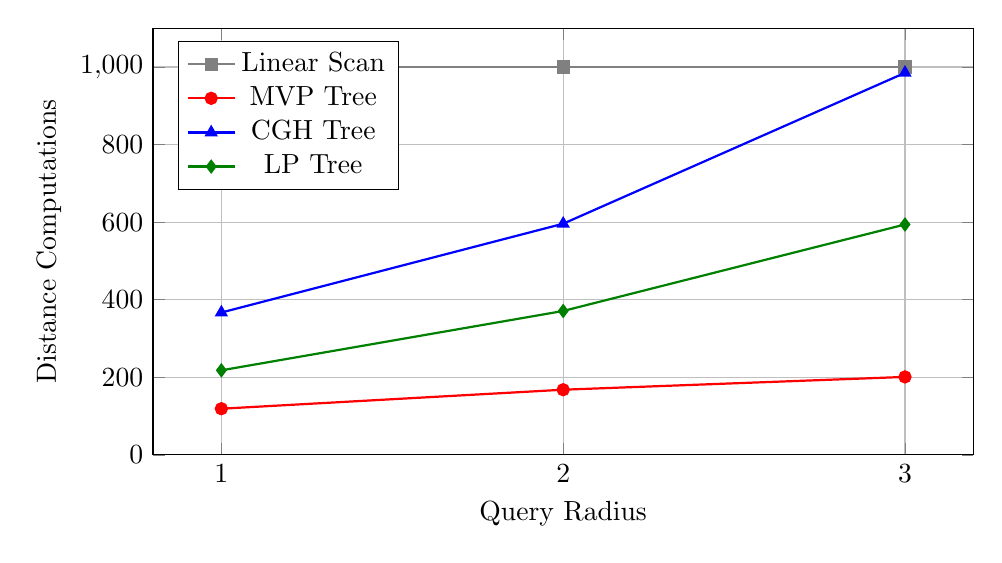
\begin{tikzpicture}
        \begin{axis}[
            width=12cm,
            height=7cm,
            xlabel={Query Radius},
            ylabel={Distance Computations},
            legend pos=north west,
            grid=major,
            xtick={1.0, 2.0, 3.0},
            ymin=0,
            ymax=1100
        ]
        \addplot[color=gray,mark=square*,thick] coordinates {(1.0,1000) (2.0,1000) (3.0,1000)};
        \addplot[color=red,mark=*,thick] coordinates {(1.0,119) (2.0,168) (3.0,201)};
        \addplot[color=blue,mark=triangle*,thick] coordinates {(1.0,367) (2.0,596) (3.0,985)};
        \addplot[color=green!50!black,mark=diamond*,thick] coordinates {(1.0,218) (2.0,371) (3.0,594)};
        \legend{Linear Scan, MVP Tree, CGH Tree, LP Tree}
        \end{axis}
    \end{tikzpicture}
    \caption{低维向量数据集范围查询距离计算次数对比}
    \label{fig:exp1-range-chart}
\end{figure}

\subsubsection{实验2:高维向量数据集}

\begin{table}[htbp]
    \centering
    \caption{实验2:高维向量范围查询性能}
    \label{tab:exp2-range}
    \begin{tabular}{lccccc}
        \toprule
        \textbf{Radius} & \textbf{Linear} & \textbf{MVP} & \textbf{CGH} & \textbf{LP} & \textbf{MVP Prune\%} \\
        \midrule
        2.0 & 500 & 73 & 140 & 73 & 85.4\% \\
        3.0 & 500 & 113 & 491 & 113 & 77.4\% \\
        4.0 & 500 & 149 & 492 & 149 & 70.2\% \\
        \bottomrule
    \end{tabular}
\end{table}

\textbf{分析}:在高维数据上,当查询半径增大时,CGH树的剪枝效果急剧下降,而MVP树和LP树仍保持较好的剪枝率。

\subsubsection{实验3:蛋白质序列数据集}

\begin{table}[htbp]
    \centering
    \caption{实验3:蛋白质序列范围查询性能}
    \label{tab:exp3-range}
    \begin{tabular}{lcccc}
        \toprule
        \textbf{Radius} & \textbf{Linear} & \textbf{MVP} & \textbf{CGH} & \textbf{LP} \\
        \midrule
        1.0 & 960 & 233 & 515 & 233 \\
        2.0 & 960 & 767 & 515 & 767 \\
        3.0 & 960 & 771 & 960 & 771 \\
        \bottomrule
    \end{tabular}
\end{table}

\textbf{分析}:蛋白质序列数据的编辑距离值域较小(0-6),导致查询半径对剪枝效果影响显著。半径为1时剪枝效果好,半径增大后剪枝效果快速下降。

\subsection{kNN查询性能对比}

\subsubsection{低维向量数据集kNN查询}

\begin{table}[htbp]
    \centering
    \caption{低维向量kNN查询性能}
    \label{tab:exp1-knn}
    \begin{tabular}{lccccc}
        \toprule
        \textbf{k} & \textbf{Linear} & \textbf{MVP} & \textbf{CGH} & \textbf{LP} & \textbf{MVP Prune\%} \\
        \midrule
        5 & 1000 & 37 & 457 & 37 & 96.3\% \\
        10 & 1000 & 51 & 538 & 51 & 94.9\% \\
        20 & 1000 & 77 & 558 & 77 & 92.3\% \\
        \bottomrule
    \end{tabular}
\end{table}

\textbf{分析}:MVP树和LP树在kNN查询上表现优异,剪枝率超过90\%。CGH树的kNN查询效果相对较差。

\subsubsection{高维向量数据集kNN查询}

\begin{table}[htbp]
    \centering
    \caption{高维向量kNN查询性能}
    \label{tab:exp2-knn}
    \begin{tabular}{lccccc}
        \toprule
        \textbf{k} & \textbf{Linear} & \textbf{MVP} & \textbf{CGH} & \textbf{LP} & \textbf{MVP Prune\%} \\
        \midrule
        5 & 500 & 433 & 500 & 433 & 13.4\% \\
        10 & 500 & 480 & 500 & 480 & 4.0\% \\
        20 & 500 & 482 & 500 & 482 & 3.6\% \\
        \bottomrule
    \end{tabular}
\end{table}

\textbf{分析}:高维数据受维度灾难影响严重,所有索引的kNN查询剪枝效果都大幅下降,接近线性扫描。

\subsection{参数影响分析}

\subsubsection{最大叶子节点大小的影响}

使用300个数据点测试不同叶子节点大小对性能的影响。

\begin{table}[htbp]
    \centering
    \caption{叶子节点大小对树结构和查询性能的影响}
    \label{tab:leaf-size-impact}
    \begin{tabular}{ccccccc}
        \toprule
        \textbf{Leaf Size} & \textbf{MVP H} & \textbf{CGH H} & \textbf{LP H} & \textbf{MVP Dist} & \textbf{CGH Dist} \\
        \midrule
        5 & 4 & 7 & 4 & 87 & 299 \\
        10 & 4 & 6 & 4 & 112 & 299 \\
        25 & 3 & 6 & 3 & 141 & 299 \\
        50 & 2 & 4 & 2 & 214 & 299 \\
        100 & 2 & 2 & 2 & 214 & 299 \\
        \bottomrule
    \end{tabular}
\end{table}

\textbf{分析}:叶子节点大小影响树高度。较小的叶子节点产生更深的树,可能有更好的剪枝效果,但也增加了节点访问开销。

\subsubsection{Pivot选择策略的影响}

\begin{table}[htbp]
    \centering
    \caption{Pivot选择策略对性能的影响}
    \label{tab:pivot-strategy-impact}
    \begin{tabular}{lcccc}
        \toprule
        \textbf{Strategy} & \textbf{MVP Build} & \textbf{CGH Build} & \textbf{MVP Query} & \textbf{CGH Query} \\
        \midrule
        RANDOM & 3810 & 5895 & 200 & 300 \\
        FFT & 6150 & 8702 & 141 & 299 \\
        MAX\_SPREAD & 25679 & 42909 & 168 & 500 \\
        \bottomrule
    \end{tabular}
\end{table}

\textbf{分析}:
\begin{itemize}
    \item RANDOM策略构建开销最小,但查询性能一般
    \item FFT策略在构建开销和查询性能之间取得较好平衡
    \item MAX\_SPREAD策略构建开销最大,查询性能不稳定
\end{itemize}

\subsection{结果分析与讨论}

\subsubsection{三种索引性能总结}

\begin{table}[htbp]
    \centering
    \caption{三种索引性能总结}
    \label{tab:performance-summary}
    \begin{tabular}{lccc}
        \toprule
        \textbf{Aspect} & \textbf{MVP Tree} & \textbf{CGH Tree} & \textbf{LP Tree} \\
        \midrule
        Build Efficiency & Medium & Higher Overhead & Medium \\
        Tree Balance & Good & Variable & Good \\
        Range Query (Low-dim) & Excellent & Good & Good \\
        Range Query (High-dim) & Good & Poor & Good \\
        kNN Query & Excellent & Poor & Excellent \\
        Large Radius Query & Good & Poor & Good \\
        \bottomrule
    \end{tabular}
\end{table}

\subsubsection{性能差异原因分析}

\textbf{MVP树和LP树}:
\begin{itemize}
    \item 使用相同的划分策略(中位数划分产生8个子区域)
    \item 剪枝条件相同,因此查询性能非常接近
    \item 具有包含规则,可以批量返回结果
\end{itemize}

\textbf{CGH树}:
\begin{itemize}
    \item 只有4个子区域,划分粒度较粗
    \item 基于距离差符号划分,平衡性依赖数据分布
    \item 剪枝条件需要$|d_1 - d_2| > 2r$才能生效,大半径时失效
    \item 没有包含规则
\end{itemize}

\subsubsection{适用场景建议}

基于实验结果,我们给出以下建议:

\begin{itemize}
    \item \textbf{低维聚类数据}:推荐使用MVP树或LP树
    \item \textbf{高维数据}:三种索引效果都一般,但MVP树和LP树相对更好
    \item \textbf{小查询半径}:三种索引效果都好
    \item \textbf{大查询半径}:避免使用CGH树
    \item \textbf{kNN查询}:推荐使用MVP树或LP树
    \item \textbf{序列数据}:根据编辑距离值域选择合适的查询半径
\end{itemize}

% Chapter 7: Conclusion
\section{总结与展望}

\subsection{工作总结}

本次Assignment 4成功完成了以下工作:

\subsubsection{代码实现}

我们实现了三种使用3个pivot的多Pivot树状索引:

\begin{enumerate}
    \item \textbf{3-pivot MVP树}:基于嵌套球形划分,产生8个子区域,具有包含规则
    \item \textbf{3-pivot CGH树}:基于距离差的超平面划分,产生4个子区域
    \item \textbf{3-pivot 完全线性划分树}:在支撑点空间中正交划分,产生8个子区域
\end{enumerate}

三种索引都实现了:
\begin{itemize}
    \item 统一的\texttt{Index}接口
    \item 批建算法(\texttt{buildIndex})
    \item 范围查询(\texttt{rangeQuery})
    \item kNN查询(\texttt{knnQuery})
    \item 统计信息收集
\end{itemize}

\subsubsection{正确性验证}

通过以下方式验证了实现的正确性:
\begin{itemize}
    \item 与线性扫描结果对比
    \item 三种索引结果相互对比
    \item 12个单元测试用例全部通过
    \item 在多种数据集上进行验证
\end{itemize}

\subsubsection{理论分析}

从理论角度分析了三种索引的:
\begin{itemize}
    \item 数据划分方式:球形划分 vs 超平面划分 vs 线性划分
    \item 支撑点信息利用:距离值 vs 距离差 vs 距离向量
    \item 剪枝能力:排除规则和包含规则
    \item 时空复杂度:$O(nk\log n)$构建,$O(k\log n + m)$查询
\end{itemize}

\subsubsection{实验分析}

在多种数据集上进行了全面的性能对比:
\begin{itemize}
    \item 低维向量数据集(2维,1000个点)
    \item 高维向量数据集(10维,500个点)
    \item 蛋白质序列数据集(960条序列)
\end{itemize}

主要发现:
\begin{enumerate}
    \item MVP树和LP树性能接近,在大多数场景下表现优异
    \item CGH树在小查询半径时效果较好,但大半径时剪枝效果急剧下降
    \item 高维数据受维度灾难影响,所有索引的剪枝效果都下降
    \item FFT是较好的pivot选择策略,在效果和效率之间取得平衡
\end{enumerate}

\subsection{主要结论}

\begin{enumerate}
    \item \textbf{多Pivot索引的价值}:使用3个pivot可以获得更多的距离信息,实现更有效的剪枝
    
    \item \textbf{划分策略的影响}:不同的划分策略对索引性能有显著影响
    \begin{itemize}
        \item 中位数划分(MVP/LP)保证平衡性
        \item 符号划分(CGH)可能导致不平衡
    \end{itemize}
    
    \item \textbf{包含规则的重要性}:具有包含规则的索引(MVP/LP)在范围查询和kNN查询中表现更好
    
    \item \textbf{维度灾难}:高维数据对所有索引都是挑战,需要更多的pivot或其他技术
    
    \item \textbf{查询半径敏感性}:CGH树对查询半径非常敏感,大半径时几乎无法剪枝
\end{enumerate}

\subsection{不足与改进方向}

\subsubsection{当前实现的不足}

\begin{enumerate}
    \item 只实现了3-pivot版本,没有支持任意数量的pivot
    \item CGH树只实现了4路划分,没有实现8路划分变体
    \item 没有实现动态插入和删除操作
    \item 没有进行磁盘版本的实现和I/O优化
\end{enumerate}

\subsubsection{可能的改进方向}

\begin{enumerate}
    \item \textbf{增加pivot数量}:研究4-pivot或更多pivot的索引效果
    \item \textbf{自适应划分}:根据数据分布自动选择划分策略
    \item \textbf{混合索引}:结合不同划分策略的优点
    \item \textbf{并行化}:利用多核CPU加速构建和查询
    \item \textbf{近似查询}:牺牲部分精度换取更高的查询效率
\end{enumerate}

\subsection{展望}

多Pivot树状索引是度量空间索引的重要研究方向。未来的工作可以从以下几个方面深入:

\begin{enumerate}
    \item \textbf{理论研究}:分析最优pivot数量与数据本征维度的关系
    \item \textbf{实践应用}:将索引应用于实际的相似性搜索场景
    \item \textbf{系统优化}:开发高效的磁盘版本索引系统
    \item \textbf{机器学习结合}:利用机器学习方法优化pivot选择和查询路由
\end{enumerate}

\subsection{致谢}

感谢毛睿教授的悉心指导,感谢大数据泛构课程提供的理论基础和实践平台。

\subsection{参考文献说明}

本实验报告参考了以下主要文献:
\begin{enumerate}
    \item Bozkaya T, Ozsoyoglu M. Indexing large metric spaces for similarity search queries. ACM TODS, 1999.
    \item Mao R, et al. On data partitioning in tree structure metric-space indexes. DASFAA, 2014.
    \item Chávez E, et al. Searching in metric spaces. ACM Computing Surveys, 2001.
    \item 毛睿. 大数据泛构(课程教材).
\end{enumerate}


\printbibliography[heading=bibliography,title=参考文献]

\end{document}
